\documentclass[a4paper]{article}
\usepackage{algorithmicx}
\usepackage{float}
\usepackage{algpseudocode}
\usepackage{graphicx}
\usepackage{vmargin}
\usepackage[utf8]{inputenc}
\usepackage{mdwlist}
\setpapersize{A4}
\setmargins{2.5cm}       % margen izquierdo
{1.5cm}                        % margen superior
{16.5cm}                      % anchura del texto
{23.42cm}                    % altura del texto
{10pt}                           % altura de los encabezados
{1cm}                           % espacio entre el texto y los encabezados
{0pt}                             % altura del pie de página
{2cm}                           % espacio entre el texto y el pie de página
\makeatletter
\setlength{\@fptop}{0pt}
\makeatother
\begin{document}
\section*{Metaheurística GRASP}
\subsection*{a) Explicación del algoritmo}
El algoritmo básicamente itera una cantidad de veces, en principio desconocida, y aplica primero la heurística golosa aleatorizada (con distintos valores de alfa). Una vez que tiene una solución factible generada por la heurística golosa aleatorizada, aplica un algoritmo heurístico de busqueda local sobre ella, obteniendo una solución nueva, mejor o igual (nunca peor). Como hay dos algoritmos distintos de búsqueda local (utilizan distintas vecindades), GRASP siempre va a elegir el mismo durante una ejecución y va a estar determinado por un parámetro de entrada.
\newline Otra cosa configurable en GRASP es quienes van a formar parte de la RCL. Considerando lo que explicamos sobre el algoritmo goloso y sus distintas decisiones y criterios, en realidad existen tres listas restrictas de candidatos:
\begin{itemize}
\item La que está conformada por los pares de nodos candidatos a ser la arista "máxima" que tome el algoritmo en la etapa inicial.
\item La que dado un nodo $u$ está conformada por los posibles pares de $u$ (ver definición de Par en la explicación de la heurística golosa).
\item La que a la hora de ubicar un nodo o un par de nodos dentro de la partición $P$, contiene los pares de posiciones que son candidatos a "la mejor manera" de ubicar los nodos.
\end{itemize} 

\vspace{0.4cm}
\noindent Estas listas de candidatos son construidas en base a tres parámetros, uno para cada una, $alfa$, $beta$, $gamma$. Cada uno de esos parámetros representa un porcentaje, que indica que tan distantes pueden estar del valor óptimo los valores contenidos en cada lista.
\newline \newline La cantidad de veces que itera el algoritmo va a estar relacionado con la cantidad de mejoras que hubo en las últimas iteraciones. Se trata de un valor entero configurable (otro parámetro, aca vamos a llamarlo $delta$), de manera tal que representa una cantidad de iteraciones. Si se hizo esa cantidad de iteraciones de manera seguida y no se observó ninguna mejora en la solución con la que se está trabajando, entonces el algoritmo termina.
\newline La solución devuelta por GRASP siempre es la mejor encontrada hasta el momento, esto significa que se va almacenando y se pisa cuando se encuentra una solución mejor.
\vspace{0.5cm}
\subsection*{a) Experimentación}
Las instancias que generamos para realizar la experimentación de la calidad de las soluciones y la performance de GRASP, fueron grafos completos. Al igual que como experimentamos con otros algoritmos, los pesos de las aristas de los grafos completos se determinaron de manera aleatoria en un rango de 0 a 50.
\newline Todas las mediciones que presentaremos a continuación se realizaron sobre el mismo conjunto de instancias, el cual tiene 100 grafos completos con vértices de 1 a 90.
\newline El objetivo de esta experimentación es poder encontrar una configuración conveniente de los parámetros de GRASP y ver si se adapta a otros grafos que no necesariamente sean completos.
\newline
\newline Vamos a presentar gráficos comparativos sobre la performance y la calidad de las soluciones que nos brinda GRASP con distintas configuraciones.
Cuando hablemos de Vecindad 1 y Vecindad 2, vamos a estar haciendo referencia al primer y segundo algoritmo de búsqueda local que presentamos.
\begin{figure}[H]
\centering
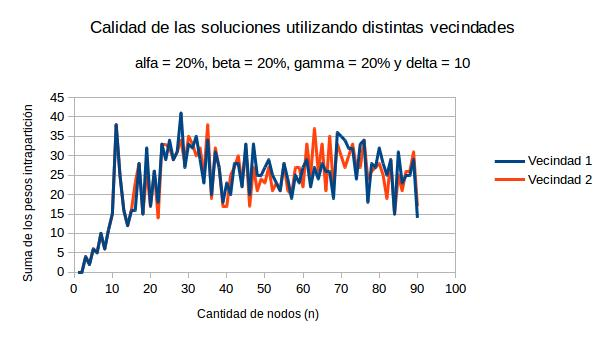
\includegraphics[scale=0.7]{20202010.jpg}\caption{En este experimento los porcentajes que determinan las RCL se mantienen bajos. También, delta es un número relativamente bajo. Podemos observar que la calidad de las soluciones que da GRASP utilizando una vecindad u otra, es similar. Solo en el intervalo de $n \in [60 .. 70]$ se puede ver que las soluciones cuando se utiliza la vecindad 1 son mejores, pero no es un rango muy significativo.}
\end{figure}

\begin{figure}[H]
\centering
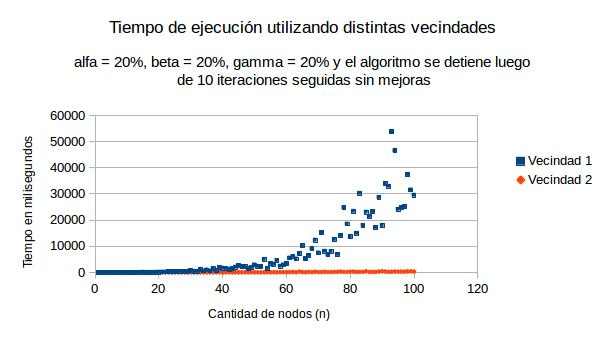
\includegraphics[scale=0.7]{20202010c.jpg}\caption{En este gráfico, podemos contemplar una diferencia significativa entre el tiempo de ejecución de GRASP utilizando una vecindad y la otra. Se puede ver incluso como esa diferencia tiende a hacerse más grande asintóticamente.}
\end{figure}

\begin{figure}[H]
\centering
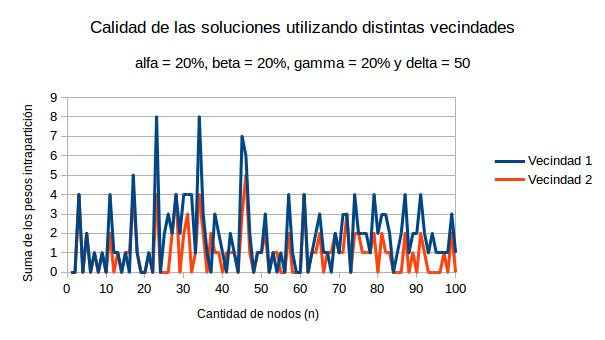
\includegraphics[scale=0.7]{20202050.jpg}\caption{
\noindent En este caso decidimos aumentar delta. Intuitivamente podríamos creer que el hecho de aumentar esto nos puede llegar a dar soluciones mejores, debido a que aumentan las chances de encontrar una mejor solución. Sin embargo, esto no paso en este caso e incluso algunas soluciones fueron peores. Esto se debe a que hay otros factores en juego además del delta (como el alfa, beta y gamma) y, como está todo aleatorizado, puede suceder que tratando de mejorar nuestras soluciones aumentando el delta, al correr nuevamente el algoritmo tengamos mala suerte y la aleatoriedad nos juegue en contra. Una vez más se puede observar que la calidad de las soluciones haciendo uso de la vecindad 1 o la vecindad 2, es similar.}
\end{figure}

\begin{figure}[H]
\centering
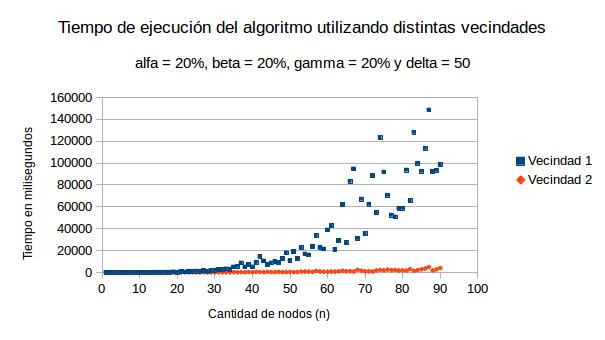
\includegraphics[scale=0.7]{20202050c.jpg}\caption{Podemos observar también como el tiempo de ejecución del algoritmo al aumentar ese parámetro, se incrementa bastante. Si bien no es del todo visible con la vecindad 2 porque el tiempo que tarda GRASP al hacer uso de ella es despreciable con respecto al que tarda cuando usa la vecindad 1, el tiempo igualmente aumenta porque, de una forma u otra estamos haciendo más iteraciones, independientemente de la vecindad a utilizar.}
\end{figure}

\begin{figure}[H]
\centering
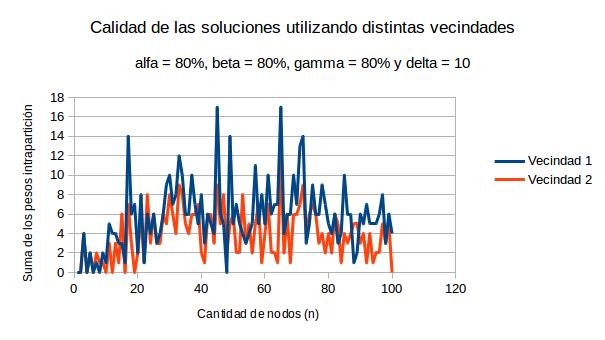
\includegraphics[scale=0.7]{80808010.jpg}\caption{Ahora, probamos aumentar bastante los parámetros alfa, beta y gamma. Lo que produce esto es aumentar el tamaño de nuestras listas de candidatos (ya que ahora podrán estar dentro de ellas los que cumplan estar hasta un 80\% lejos del mejor). Vemos que las soluciones que provee GRASP utilizando una vecindad u otra, siguen siendo similares en cuanto a calidad. Empezamos a pensar que esto es independiente de los valores de alfa, beta y gamma.}
\end{figure}

\begin{figure}[H]
\centering
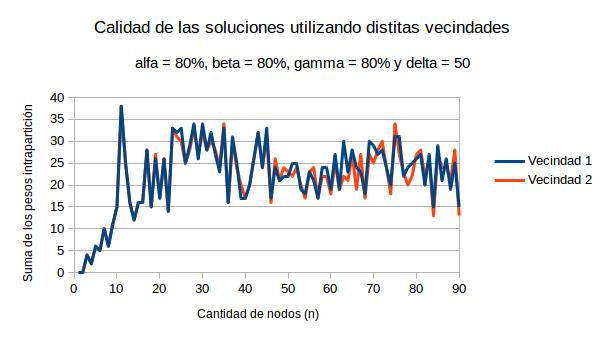
\includegraphics[scale=0.7]{80808050.jpg}\caption{Una vez más, aumentamos el delta y vemos que, con ninguna de las dos vecindades hay una mejora realmente notable, la cual justifique el costo necesario para realizar este cambio.}
\end{figure}
\noindent Dado que las soluciones que provee GRASP haciendo uso de cualquiera de las dos vecindades son muy similares en cuanto a calidad, al parecer lo que nos conviene hacer es utilizar la vecindad 2. Esto es así debido a que las soluciones que produce GRASP con la vecindad 2 son muy similares a cuando utiliza la vecindad 1, pero con un tiempo de ejecución muchísimo menor.

Como los experimentos realizados tienen siempre el mismo valor para alfa, beta y gamma, sería interesante ver si las soluciones que provee GRASP utilizando valores más distantes (y por ende distintos) de alfa, beta y gamma, siguen siendo similares con una vecindad u otra, en términos de calidad.
\newline Para ver esto realizamos una última experimentación, con distintos valores de alfa, beta y gamma:

\begin{figure}[H]
\centering
\includegraphics[scale=0.7]{ultimaexp.jpg}\caption{Vemos que, salvo casos muy particulares, las soluciones con una vecindad u otra siguen siendo similares a pesar de que alfa, beta y gamma ahora no comparten el mismo valor (y son notablemente distintos).}
\end{figure}

\begin{figure}[H]
\centering
\includegraphics[scale=0.7]{ultimaexpc.jpg}\caption{Acompañamos al gráfico anterior, con éste que nos provee alguna información sobre los tiempos de ejecución con los valores anteriores. Se puede ver que los tiempos son similares a cuando alfa = 80\%, beta = 80\%, gamma = 80\% y delta = 50.}
\end{figure}

Finalmente, podemos concluir que una buena configuración de los parámetros de GRASP puede ser tomar valores de alfa, beta y gamma relativamente bajos (20 puede ser un buen número según nuestros gráficos), ya que al parecer, no tiene mucho sentido agrandar demasiado el tamaño de nuestras RCL's si lo que buscamos es mejorar la calidad de las soluciones. Por otra parte, el valor del delta tampoco necesita ser grande (10 podría ser un valor razonable según el primer gráfico). Finalmente, es claro que es conveniente utilizar la vecindad 2, ya que solo se poseen dos vecindades distintas y GRASP con cualquiera de ellas arroja soluciones similares a las que daría si utilizara la otra, con la diferencia de un tiempo de ejecución significativamente menor.
\end{document}